\chapter{State of the art}

\section{Videospiel-Markt}

Videospiele sind Bestandteil des Medienkonsums in Deutschland. Rund 6 von 10 Menschen in Deutschland spielen Computer- und Videospiele. Der deutsche Videospiel-Markt machte mit Videospiel-Hardware, Videospiel-Abo-Diensten und Videospielen im Jahr 2023 einen Umsatz von 9,97 Milliarden Euro. Dabei machten Videospiele und In-Game K�ufe mit 5,845 Milliarden Euro einen Umsatz von ca. 59\% aus. Im Vorjahr 2022 entstand ein Umsatz von 9,432 Milliarden Euro, somit stieg der Umsatz von 2022 im Jahr 2023 um 6\%.  Zahlen f�r das Jahr 2024 sind noch nicht bekannt.

\begin{figure}[h]
  \centering
  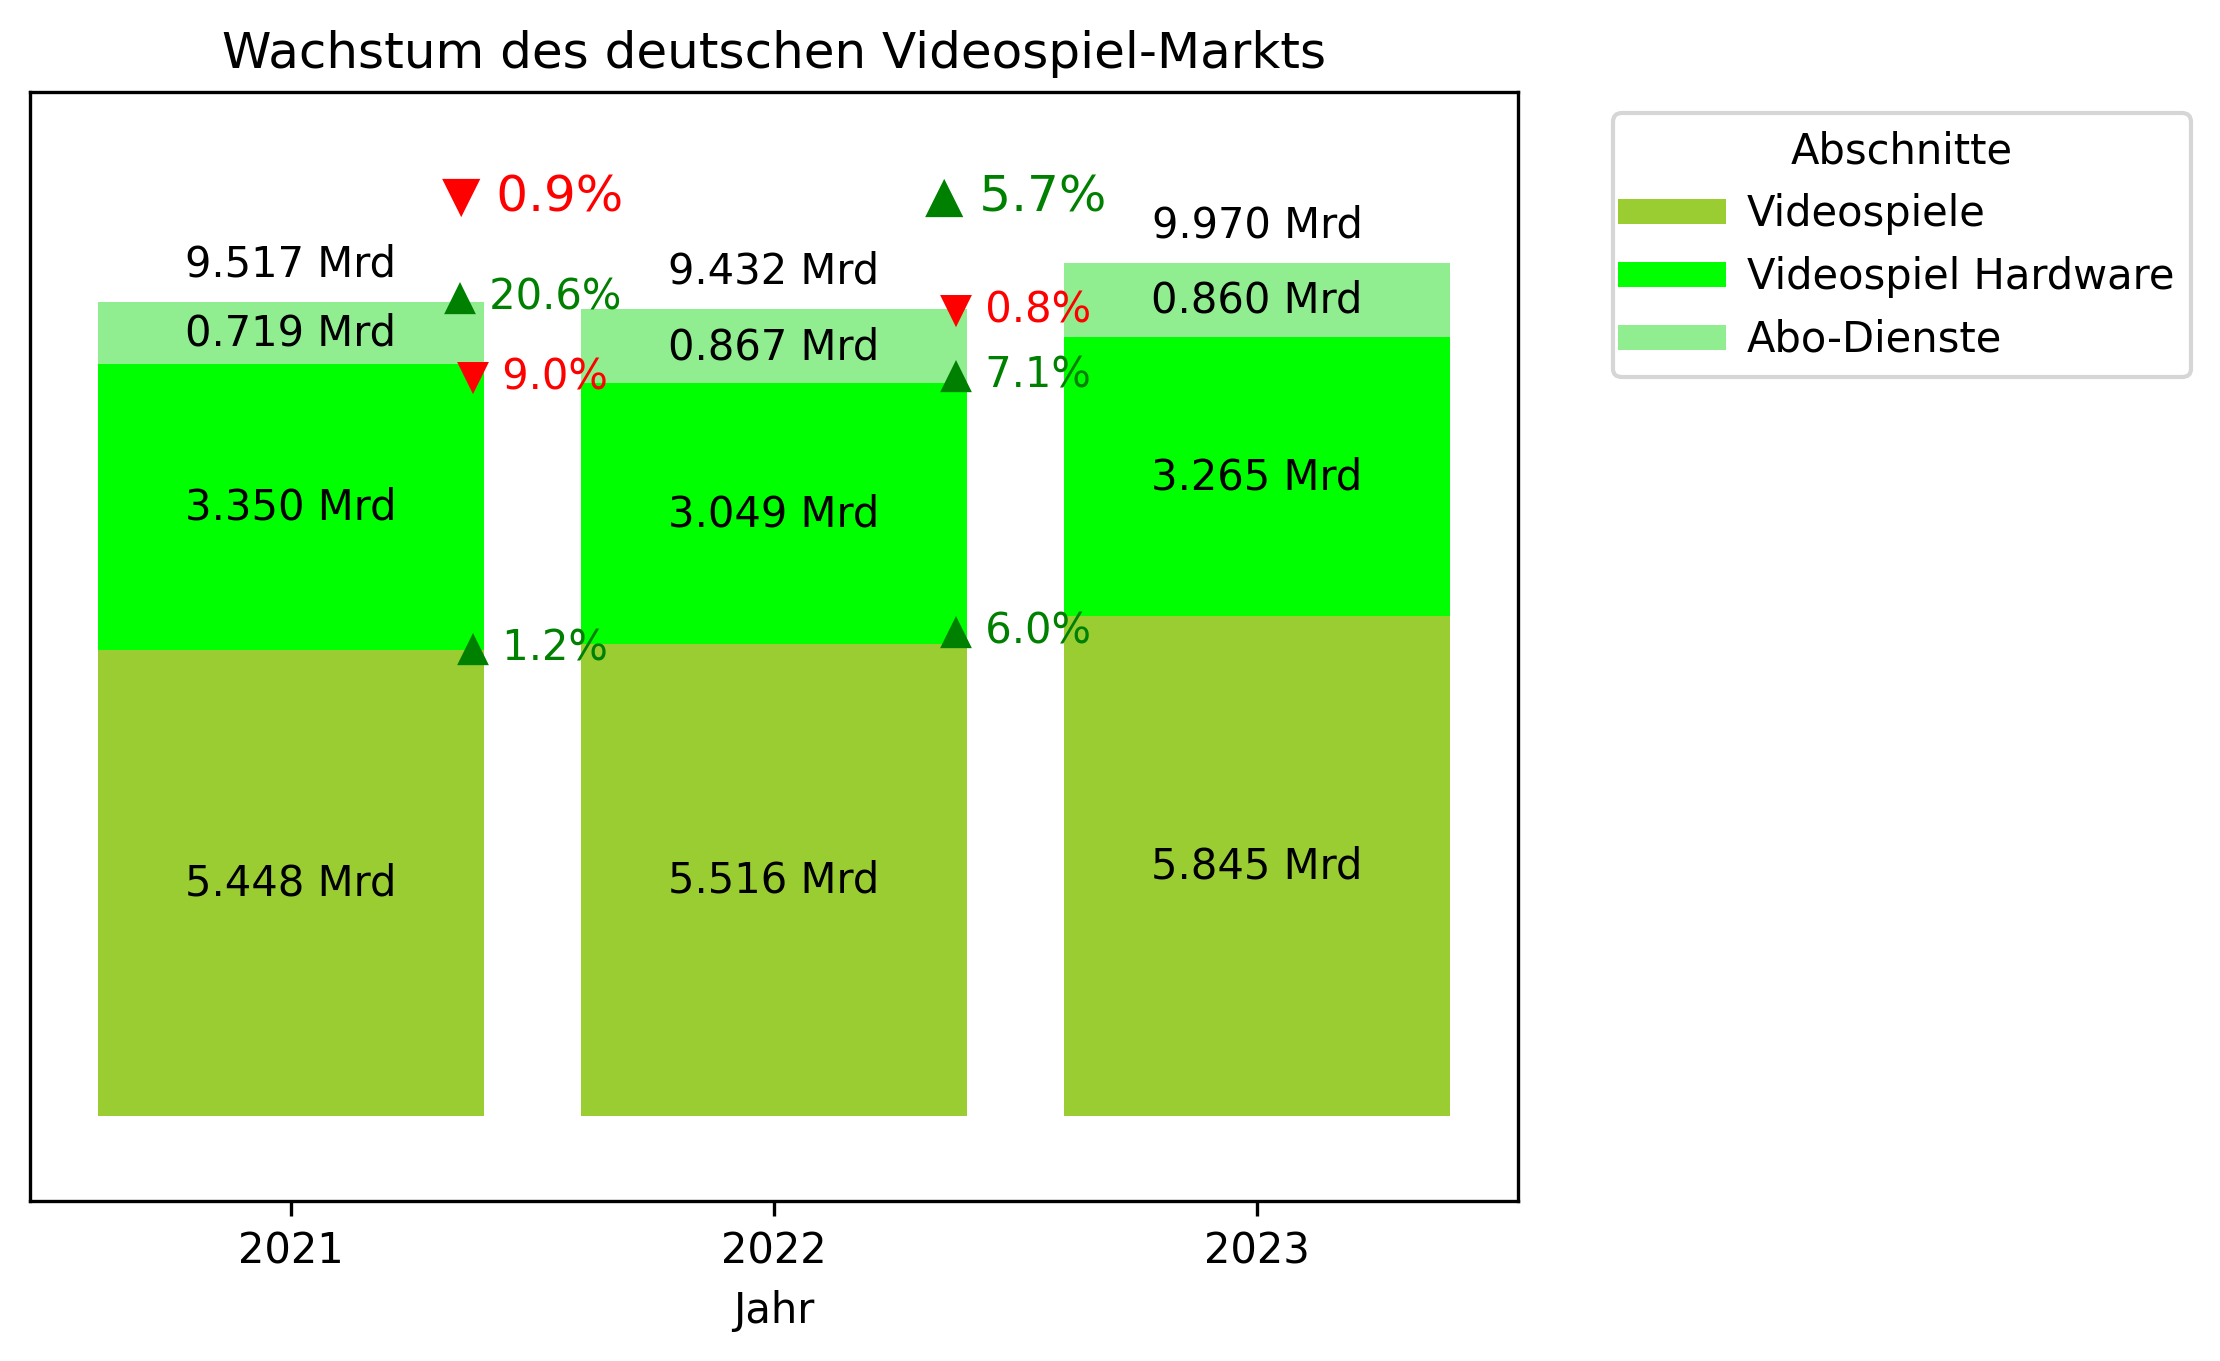
\includegraphics[width=15cm]{state_of_the_art/deutscher_vs_markt}
	\captionsetup{justification=justified, format=plain}
  \caption{Wachstum des deutschen Videospielmarkts �ber die Jahre}
  \label{Deutscher Videospielmarkt}
\end{figure}

Auf der erfolgreichen Computerspiel Vertriebsplattform Steam von Valve wurden vergangenes Jahr 2023 14.324 Computerspiele ver�ffentlicht. Seit 2019 w�chst die Ver�ffentlichung der Computerspiele auf Steam stetig.

\begin{figure}[h]
  \centering
  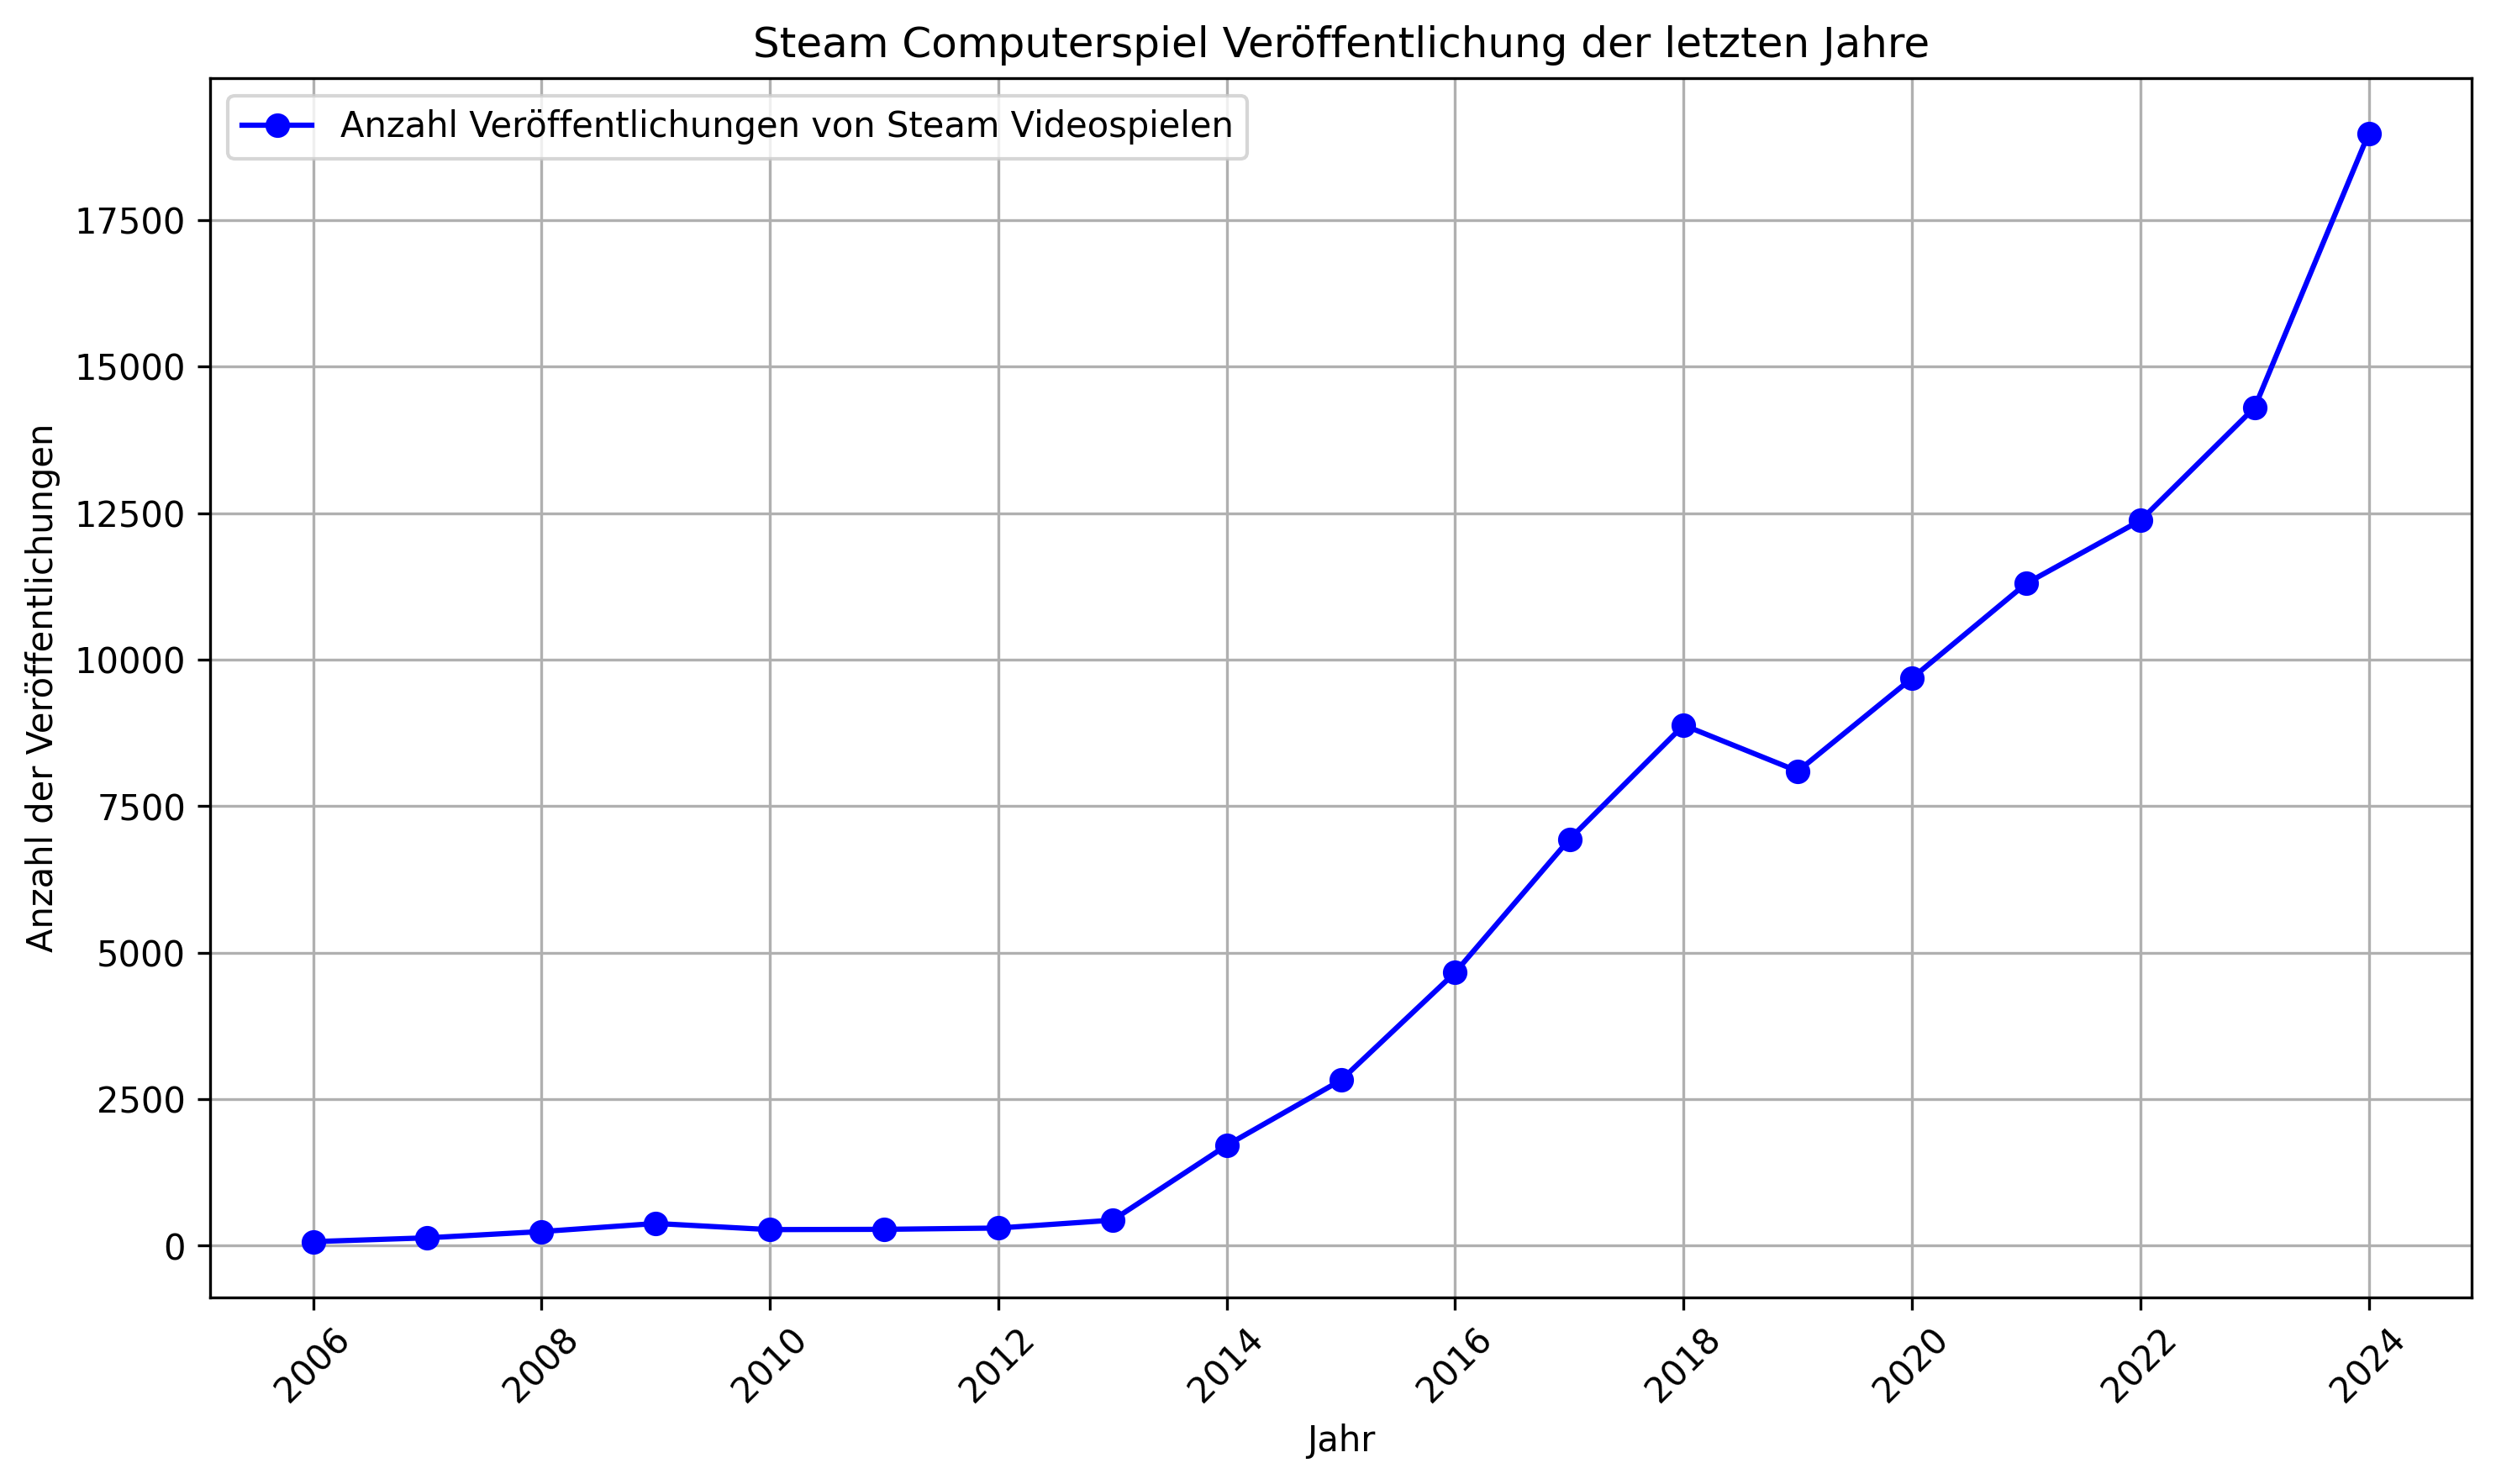
\includegraphics[width=15cm]{state_of_the_art/steam_veroffentlichungen}
	\captionsetup{justification=justified, format=plain}
  \caption{Computerspiel ver�ffentlichungen auf Steam �ber die Jahre}
  \label{SteamDB Statistik}
\end{figure}

Folglich kann davon ausgegangen werden, dass es Stakeholder gibt, die sich f�r Videospiele interessieren.


\section{Entscheidungssysteme in der Game AI}

Es wurden bereits Entscheidungssysteme, wie Behavior Tree (BT), Finite State Machine (FSM) und Goal Oriented Action Planning (GOAP) in ihrer Funktion beschrieben. Das folgende Kapitel widmet sich der Analyse und Erl�uterung der Anwendung dieser drei Entscheidungssysteme in der modernen Videospielentwicklung. 

%Fortsetzung
\subsection{Fortschrittliche Methoden des maschinellen Lernens}

Der Trend von fortschrittliche Methoden des maschinellen Lernens, hat an Bedeutung gewonnen. Die Methoden spielen zwar eine immer gr��ere Rolle im allt�glichen Leben, haben jedoch einen eher geringeren Einfluss auf die Game AI. Diese Methoden erfordern gro�e Mengen an Daten f�r das Training und es ist �u�erst schwierig, sie auf unvorhergesehene Situationen zu testen. 

Es existieren wenige ver�ffentlichten Studien, die ihre Anwendung als Entscheidungssystem f�r NPC dokumentieren, daher werden diese im Schwerpunkt nicht weiter betrachtet. Es w�re jedoch interessant diese Methoden ausf�hrlicher in der akademischen Forschung Richtung Game AI zu sehen.

Die Methoden des maschinellen Lernens kann man in supervised learning (SL), unsupervised learning (UL) und reinforcment learning(RL) unterteilen. So bekommt SL gelabelte Daten und UL Rohdaten mit denen sie trainieren. W�hrend RL auf Basis der Umgebung lernt und durch richtige Aktionen belohnt wird. So wird Deep Learning, ein Teil von SL, f�r Spracherkennung und natural language processing benutzt. Im Strategiespiel StarCraft wird RL f�r das \textit{micromanagement} der NPC benutzt. \autocite{inbook}

Die Evolution�re-Algorithmen sind inspiriert durch Darwins Theorie der Evolution. Sie optimieren dabei eine Population, wo jedes Individuum eine L�sung repr�sentiert und mit einer Fitness-Wert gekennzeichnet ist. Durch Iterationen finden Selektionen und Mutationen in der Population statt, welche den Fitness-Wert der optimalen L�sung erh�hen. Im Bereich der Videospielentwicklung optimierte der Algorithmus beispielsweise die Baureihenfolge der NPC im Strategiespiel StarCraft. \autocite{inbook}

\subsection{Finite State Machines}
In den fr�hen Tagen der Spieleentwicklung waren FSM ausreichend, um eine Entscheidungsmechanik f�r NPCs bereitzustellen. Klassiker wie Pac-Man und Sonic the Hedgehog nutzten FSM, um das Verhalten ihrer NPC zu definieren. Auch FPS, wie etwa Half-Life, haben FSM als Entscheidungssysteme genutzt. 

%Ein wesentlicher Nachteil von FSM besteht darin, dass die Anzahl der �berg�nge exponentiell ansteigen kann, wenn die Anzahl der Zust�nde zunimmt. Dieses Problem l�sst sich in gewissem Ma�e durch den Einsatz von hierarchischen FSM (HFSM) reduzieren. Dennoch neigt eine FSM dazu, in bestimmten Situationen ungenau zu reagieren, beispielsweise wenn Zust�nde oder �berg�nge unvollst�ndig definiert sind. Au�erdem k�nnen Leistungsprobleme auftreten, insbesondere bei einer �berm��igen Anzahl von Zust�nden.

%Diese Einschr�nkungen f�hrten dazu, dass die Spieleindustrie nach alternativen Methoden f�r die Entscheidungsfindung von NPCs suchte. Ein Beispiel hierf�r ist GOAP von Jeff Orkin, welches einen neuen Ansatz durch einen Suchalgorithmus entwickelte.

\subsection{Behavior Trees}
- BTs have become a popular tool for developing the decisions of NPC characters. Halo 2 (Yannakakis and Togelius 2018) was one of the first modern games that used BTs
- Panwar discussed the difficulties the developers faced when developing the AI for the game The Last of Us
- the authors explained that they used BTs and FSMs together to create a decision-making tool for NPCs in the game Final Fantasy XV which they call AI Graph Editor.
- With recent technological developments, FSMs, DTs and BTs for managing decisions of NPCs are deficient in some situations, such as bad performance on overgrown tree structures, repeating mistakes without learning, and selecting the same decisions without being adaptive to different conditions creating the need for more believable character management methods
- Researchers use complementary techniques such as employing reinforcement learning or genetic algorithms to overcome these shortcomings in earlier methods.

\subsection{GOAP}
